\documentclass[12pt,a4paper]{article}
\usepackage{ucs}
\usepackage{caption}
\usepackage[latin1,utf8x]{inputenc}
\usepackage{amsmath}
\usepackage{caption}
\captionsetup{font=small,labelfont=bf}
\usepackage[danish]{babel}
\usepackage[rmargin=3cm,tmargin=3.3cm]{geometry}
\usepackage{listings}
\usepackage{color}
\setlength{\parindent}{0pt}
\setlength{\parskip}{1ex plus 0.5ex minus 0.2ex}
\usepackage{graphicx}
\usepackage{fixltx2e}

\usepackage[T1]{fontenc}
\usepackage{textcomp}

%insert links
\usepackage{hyperref}
\usepackage{xcolor}
\definecolor{dark-red}{rgb}{0.4,0.15,0.15}
\definecolor{dark-blue}{rgb}{0.15,0.15,0.4}
\definecolor{medium-blue}{rgb}{0,0,0.5}
\hypersetup{
    colorlinks, linkcolor={dark-red},
    citecolor={dark-blue}, urlcolor={medium-blue}
}
\usepackage{fancyhdr,lastpage}	
\pagestyle{fancy}


\definecolor{mygreen}{rgb}{0,0.6,0}
\definecolor{myblue}{rgb}{0,0,1}
\definecolor{myyellow}{rgb}{0.7,0.7,0}
\definecolor{myblack}{rgb}{0,0,0}

\lstset{
	basicstyle=\ttfamily\footnotesize
	breaklines=true,
	numbers=left, 
	commentstyle=\color{mygreen},
	stringstyle=\color{myyellow},
}

%header
\lhead{ 
	Embedded Systems A2\\
	02131 \\ 
}
\chead{ 
}
\rhead{ 11 November, 2013 \\ \bigskip  }

%Footer
\lfoot{
	\rule{\textwidth}{0.1mm}\\
}

\cfoot{}
\rfoot{\ \\ \scriptsize{Side \thepage\ af \pageref{LastPage}}}

\begin{document}

%Forside
\begin{titlepage}
	\begin{center}
		\vspace*{13\baselineskip}
		\huge
		\bfseries
		Embedded Systems\\ 
		\ \\
		02131 \\[5\baselineskip]

		\normalfont
		\Large
		R-peak detection. \\
		Assignment 2\\	
		2013

		\small
		\vfill
	\end{center}	
	\begin{flushleft}
		Jakob Welner, s124305\\
	 	Jacob Gjerstrup, s113440\\
	\end{flushleft}
\end{titlepage}

\ \\
\section*{Abstract}
The task of this assignment was to implemented, integrate and analyse a co-processor. This co-processor would be taking care of a very specific task that was identified by analysing what ``good performance'' means for this task. It was be implemented in such a way that it could communicate with a processor through a bus, the processor being the master and the co-processor being the slave. Once it was implemented and integrated, its performance were analysed to determine the improvement in performance, thereby finding out that it does not have ``good performance'' as defined earlier - it is actually slower than the single-processor setup.\\

\thispagestyle{empty} 
\newpage

%Table of Contents
\tableofcontents
\thispagestyle{empty} 
\newpage

%Reset pagecount
\setcounter{page}{1}

%Alm. sider
\
\section{Introduction}
	After successfully implementing and integrating a dedicated processor to take care of the MWI filter, Medembed wants a co-processor implemented and integrated into the same system. The task of this co-processor would be to further optimize the algorithm, letting the processor created in A2 take care of the more general tasks while the co-processor takes care of a very specific task with a minimum of power, time and size required.\\
	This co-processor were to be implemented in Gezel like the initial processor, and this report will discuss precisely how this co-processor were developed and integrated. It will also discuss what is most important in terms of performance, that is, whether the co-processor is implemented with optimizing speed, power or size in mind.
	
\subsection{Requirements}
Below follows a list of functional and non-functional requirements:

\textbf{ Functional requirements for the application:}
\begin{itemize}
	\item A co-processor must be designed. This co-processor must be analysed in terms of:
	\begin{itemize}
	\item Functionality
	\item Communication interface
	\item Performance (Speed, area and power)
	\end{itemize}
	\item The co-processor must be implemented and integrated into the system with the processor and RAM
	\item The co-processor must communicate with the processor and RAM through a bus.

\end{itemize}
\textbf{Non-functional requirements for the application:}
\begin {itemize}
	\item The co-processor must be implemented with the use of Gezel
\end{itemize}

\section{Analysis}
 	In order to initiate the structure- and design-process of the program, a number of questions needed to be answered first:
 	
 	\begin{enumerate}
	\item How do we define ``good performance''?
	\item What functionality should the co-processor have?
	\item How should the co-processor communicate with the rest of the system?
	\item How can the co-processor be implemented?
	\item How can the co-processor be integrated into the system?

\end{enumerate}

\subsection{Problem 1: Defining good performance}
\label{Prob1}
	The first thing that should be done would be to analyse the co-processor in terms of what good performance is. In terms of performance, there are three areas to consider, and these are: High speed, low area and low power. The task was to decipher which was more important for the current project, as each has a distinct impact on the co-processor.\\
	
	\subsubsection{Speed}
	In order for the system to process the sensor data without falling behind, a certain speed is required. However, speed of a processor is usually dependent upon the task at hand and can be defined in two ways. One is by clock frequency, where the system can handle so and so many instructions per second. The other is by the complexity of instructions that the system can handle per clock. For a general purpose CPU the complexity of the processes being run can vary arbitrarily. This makes it difficult to specifically define it's speed in general. Until lately the CPU manufacturers have defined their CPU speeds in clock frequency. More modern systems have now started optimizing the instruction complexity instead as well as spreading the load over several cores where each individual core isn't necessarily running at high clock frequencies. 
	In the case of this project, the minimum speed required was defined as being able to process 250 samples each second. For this particular case, the process is running on dedicated hardware on a well defined datapath and the only variable is the size of the input. The instruction set is specifically made for this one task and the hardware is designed to process the task as efficiently as possible. A situation like this leaves it up to the hardware designer whether to focus on complex instructions or fast clock frequencies and the definition of speed is relative to all the alternative design decisions. The fact that this project is about designing a co-processor introduces a speed relative to the communication with the master CPU. Given that the whole chip will most likely run at the same clock frequency and the fact that the clock cannot tick before all signals have reached their destination, it is crucial that the co-processor does not introduce the longest critical path. Otherwise the whole system clock will have to be slowed down, which in turn will slow down all the processes of the CPU. With this in mind, the speed of the co-processor will be defined by throughput per clock-cycle, while keeping the datapath shorter than the critical path of the CPU.\\
	\subsubsection{Power}
	Power is important as it will either have the impact that the user will need to charge the battery more often, which will be a bother, or that the size of the battery will increase, thus increasing the total size of the device.\\
	To measure the power of a chip, three values can be considered - the first is switching, which is the amount of power used because of active components; the second is short-circuit, which is when both pMOS and nMOS are on at the same time; and the final value is called static and refers to power supply due to inactive components. This report will focus mainly on switching, as this value rise proportionally with activity, and this can be measured by looking at the amount of toggles that happens within a program - that is, the amount of signals switching from 0 to 1 or from 1 to 0.\\
	
	\subsubsection{Size}
	Finally, size is important as the larger the co-processor is, the larger the whole unit will become. Size can be measured by simply counting the amount of components and bit widths and adding all these together. Having a small chip-size is beneficial for many reasons. Financially, producing larger chips will limit the amount of chips that can be fitted on each silicon wafer. With a set prize and size of such wafers, the cost of each chip will raise with the area. Furthermore, given the probability of impurities and faults on each wafer, the larger area will also lead to a larger possibility of each chip containing such faults. Area is usually one of the primary limitations when designing a chip. Most design decisions are generally made based on the allowed area. If the minimum area is easily met, the chip can be optimised further in terms of power by using the spare area to duplicate modules that are accessed by multiple places, thus shortening the route to reach those modules.

\subsection{Problem 2: Functionality of the co-processor}
	Once the choice of performance requirement had been chosen, the next task was to decide how to actually optimize the co-processor in terms of that specific task. There were two ways to implement equation 1 \footnote{See \cite{A3}, page 2 for the equation} :\\
	One way was to sum all the values first and then divide with N. The other was to divide every valuable with N before summing them up. Both ways are correct, mathematically speaking, but the way each calculation is done is very different, and it would be important to identify the benefits and issues with choosing one over the other in regards to the choice of performance requirement.\\
	
\subsection{Problem 3: Communication of the co-processor}
	The next task was then to identify a suitable communication interface. This interface had to be able to handle transferring of the filtered data from the memory to the co-processor, as well as a way of deciding when the co-processor should begin and stop executing.\\
	The task here was then to define the above, and furthermore, to prepare a list of commands that the co-processor would be able to decode and execute to do the calculation of the equation. For this it was needed to make a block diagram of how exactly the communication interface would work.

\subsection{Problem 4: Implementation and integration of the co-processor}
	Once the previous steps had been taken care of, the next part was to then implement the co-processor and subsequently integrate this into the system developed in A2. The actual implementation of the separate unit was very straight forward and thus did not give any problems, but the integration with the Platform turned out to be more troublesome.\\

\section{Design}



	
\section{Implementation}
\subsection{Good Performance}
	\subsubsection{Speed}
	Speed remains important as the processor must be able to process the necessary 250 data points per second that the sensor picks up, as if it cannot manage this, the incoming data will be delayed more and more, and the user will be shown old data. However, once this threshold has been passed, speed becomes the least important part, as if it runs much faster than necessary, it will simply idle as it waits for data points, wasting power on nothing. This report deems speed to be the most important, at least up to the point where it can calculate 250 data points per second, simply because the processor must be able to do these calculations and the harder it is to do these calculations, the larger the processor will be (increasing size) and the more power it will require (increasing power consumption). The opposite naturally also holds - the faster the processor is beyond 250 data points, the smaller it can be made, and the lower the clock frequency can be set, thus reducing both size and power.\\
	
	\subsubsection{Power and Area}
	Opposite speed, power and area both remains unimportant until the threshold of 250 data points has been reached, at which point they become much more important. Furthermore, as was documented in A2, reaching 250 data points per second in terms of speed is not a hard feat, and as such, for the purpose of defining what \"good performance\" means, power and area remains more important than speed.\\
	\\
	Of these, this report deems that power remains slightly more important for the following reasons:\\
	\begin{enumerate}
	\item If the processor is too big, the ECG scanner becomes unwieldy and cumbersome, not to mention that current manufacturing processes of general purpose processors are now able to make the devices very small, making it harder to justify why a dedicated chip should be produced.
	\item If the device requires too much power, the processor will either need to be charged more often (which a user can live with, but it is bothersome) or, if taken further, the user might need to change batteries in the middle of the day. The alternative is to increase the size of the battery to make up for the power consumption, but as that increases the size of the device, the risk is that it becomes too unwieldy and cumbersome to use in a day-to-day life.
	\end{enumerate}
	Therefore, optimizing in terms of power will both keep the power consumption down and keep the battery from requiring too much space, thus not increasing the size of the device.\\
	
\subsection{Functionality of the co-processor}
	\label{Functionality}
	With the considerations above in mind, the functionality of the co-processor should now be defined. This report decided to only divide after everything has been summed up, as having a division for each value to be summed would not only slow the processor down greatly (A division involves a multiplication and a bitshift, and whereas a bitshift is quite fast, a multiplication is not), it would also mean more mathematical operations per data sample, which in turn would mean the amount of toggles would be higher, thus increasing the power consumption as well.\\
	\\
	Furthermore, as in A2, it was decided not to sum up all 30 values for every single data point - instead, a variable will hold the value of the 30 previous points and when a new data point is loaded, it will be added to the summation variable and the value that goes 30 data points backwards will be subtracted. This means that instead of adding 30 variables, all that needs to take place is a single addition and a single subtraction, and since addition and subtraction are almost equally as fast, this is certainly a benefit, speed wise. Furthermore, it also cuts down on the amount of toggling, as the processor only needs two points, rather than 30, to do the calculations.\\
	\\
	The above is made possible by sending all data in a single 32 bit signal over the bus - this report assumes that no value exceeds 16 bit size, which is equivalent to that no value exceeds $2^(16) = 65536$. This assumption comes from the fact that in all the data used for this report, no value exceeds the threshold of 10.000. Since the data signal will be 32 bit nevertheless, though, 16 bit were chosen both to use all 32 bits and furthermore, to ensure that even if the data suddenly peaks dramatically, the sensor will have the capacity to handle this.\\

	%Skal m�ske rykkes til performance analysis senere
	
		
\subsection{Communication of the co-processor}
	From A2 it was found that the actual Moving Window Integration could be done fairly easy by approximating the division of 30 by a multiplication and a bitshift. The operations were performed on the sum of the past 30 samples. The sum of the samples was maintained by an accumulator over the past 30 values and for each cycle the latest value was added and the value 30 samples old was subtracted. Using the same system for the coprocessor, the datapath could end up being very simple. The only data needed would be the latest sensor value and the old value, with the accumulator being internal in the coprocessor. For the coprocessor to react properly to commands from the CPU, it would furthermore need an input for different states. As the data and command needed to be sent across the BUS, a protocol needs to be established for the communication, partly by new assembler commands and partly by a moderating the existing CPU circuit.

	\begin{figure}[h!]
		\centering
			\includegraphics[width=1\textwidth]{Screenshots/CPU og coprocessor.png}
		\caption{The Design diagram of the CPU}
		\label{DesignDiagram}
	\end{figure}

\subsection{Implementation and integration of the co-processor}
	First thing to do was to build the coprocessor. Given the very simple math and the moving sum, the whole MWI operation could be performed in a single cycle. Furthermore it could be written as a single datapath with combinatoric logic. Given that the coprocessor would run at all times as well as needed a way to reset the accumulator before start, it had to support 3 different states; Idle (maintain accumulator sum and do nothing), reset (clear accumulator register) and run (receive datapoints, perform MWI calculations and return data). With the premade Platform and BUS supporting a command- and data-signal to be sent, the data needed for the MWI should be maintained in those two. For setting the states of the MWI only 2 bits were needed. This signal could easily be contained in the command signal, whose only requirement from the bus was to reserve the 4 first bits for TargetID. Figuring which state to send when was a different issue though. For this a new opcode needed to be constructed for the CPU. As suggested in the A3 guide a "Send Command" would be a good way to do it. In the case of this assignment 3 crucial inputs were needed; Where to store the output, where to get the newValue and where to get the oldValue to pass on to MWI. Furthermore, making the send command (SCMD) a little generic it should in theory be possible to extend it to communicate with multiple coprocessors at a later stage. Therefore it needed to contain the id of the coprocessor as well. 
	Finally, the command should be able to distinguish between resetting the MWI coprocessor and running it. It was decided to handle this by implementing it in the form of: SCMD mwi\_reset to reset the MWI coprocessor, and SCMD mwi\_run R1 R2 R3 in order to run the MWI filter, where R2 is the newValue, R3 the oldValue and R1 the place to store the filter output. In order to decode this and format it to hex-code for the instruction memory, the assembler.py script was extended. Adding a new assembler command was easy but the fact that this one included further data in the sense of 2 choices for the MWI state, this data had to be put somewhere that would fit in the current CPU circuit.
	Wanting to keep the structure of the CPU controller, every command should only have a single case. To add another opcode as well as adding the extra 2 bits of data turned out to go beyond the 5 bits used for opcodes in A2. In order to fix this, the opcode-length was extended to 6 bits and the SCMD was implemented as the only command setting the 6th bit high. This meant that the opcode had another 5 bits free for unique states so the mwi states was defined as the 1st and 2nd bit in the opcode, when the 6th bit was high. With this set the controller could match the SCMD by simply looking at the 6th bit but passing on the first 2 bits to the sfg related to SCMD. Those to state bits could then be included in the bus\_cmd in the sfg and the signal could be sent. 
	Implementing the data for MWI without loosing precious cycles on bus transfers, it was needed that 2 values were sent simultaneously in the data-signal. To do this another state in the ALU was added, that would take the values of register A and register B, cast them to 16 bit values and stick them together, one after another in a 'collapsed' 32 bit signal. This could be done due to the assumption that there wouldn't occur any input numbers beyond the limit of 16 bits. In this way it was possible to send the MWI state as well as 2 values during a single BUS transaction. Due to the data from the CPU to the bus not previously going through the ALU, a final state was added to the ALU, that simply passed on the value of A to the output. In this way rewiring the CPU so that the data-signal from the CPU to the bus came from the ALU instead of MUX1, the data could come through.
	On the slave-side of the bus, the coprocessor was based on a copy of the DataMemory datapath. All signals and registers concerning DataMemory were copied and renamed for coprocessor - prefix: CP and COP. The coprocessor datapath in itself only needed to handle BUS communication and then split up the received signals to pass on to the MWI dp in the correct format. Initially when executing the system following the 30th sample the process would get caught in a loop of NOP. After extensive research and analysis of the signals it was found that the issue occured when executing a LOAD command immediately followed by a SCMD. This was due to the BUS needing another cycle to reach ready-state after returning a value from LOAD. Too fix this a NOP was added between the LOAD and SCMD mwi\_run R5 R1 R2, line 7 and 9 (for 0-based numbering). With this fix the system was running.	
	
\section{Performance analysis}
\label{Performance Analysis}
	As can be seen in the output of which commands are run when during the course of the calculations (\ref{Commands}), it can be seen that every time a LOAD command is initiated, 8 NOP (No-Operations) follows, each taking a single clock cycle. This clearly shows that Load commands do take a lot of time and calculation and therefore, reducing them as much as possible was crucial if the processor were to reach the computation power necessary to calculate 250 data points per second. Furthermore, the list of commands also shows that communication on the bus also takes 8 clock cycles (as seen by looking at the command SCMD and the following 8 NOP commands carried out before the next calculation) - this is clearly another slow process that should be optimized as much as possible if the processor were to reach its target, speed wise.\\ %699 nops contra 301 rest
	Interestingly enough, out of a 1000 clock cycles, 699 clock cycles were spent on waiting for LOAD commands or bus communication, and only 301 clock cycles were spent on actual calculations, clearly showing just how much time it actually takes to communicate over the bus.\\
	\\
	The above, however, is not something that will be optimized upon in this report, as the time needed to do the LOAD commands are decided upon by Gezel and the fact that the co-processor must work on the bus means both must run their due courses. The rest of the operations, however, can be optimized and analysed. These 301 clock cycles consist of sequences of $1 addition \rightarrow 1 subtraction \rightarrow 1 multiplication \rightarrow 1 bitshift$. In total, each sequence only takes a single clock cycle due to the fact that both additions, subtractions and bitshifts are very fast operations. Furthermore, this report does not require any looping through values, as described in section \nameref{Functionality}, thus making the actual critical path very short.\\
	%Skriv noget om tidsm�ngden kr�vet til at lave Critical Path
	\\
	In terms of size, this report has done very little to optimize it, but the size of the processor still remains very small as there are no loops in the co-processor, nor are the 30 previous values actually stored. As such, the size of the co-processor is equal to the sum of the bit size of every signal used in the co-processor, and in total, that amounts to $7*32+2*16+2+5*1=263$ bits which remains very small in the modern age where processors commonly has several megabytes of intern memory \cite{CoreI5}.
	\\
	Finally, in terms of power, the interesting thing to look at is the amount of toggles - these can be seen on \ref{Toggles}. What this tells is, first of all, that it took 8606 cycles to calculate 250 data points. Secondly, it shows the amount of evaluations and toggles per operation. The names of the operations are assigned by Gezel itself and cannot be used for much - what is interesting, though, is the amount of toggles done. To use these for anything, they should be summed up, which in total gives: $203641+108889+168244+291862+11242+18401+495+25999+1502+830+2319+803+197736+62190+3442+2168+19539=1.119.302$ toggles. This is equal to the value P\_Switching, which can be used in the formula to calculate the average power usage of the system with the following formula: P\_avg = P\_switching + P\_short-circuit + P\_static. For the purpose of this report, it is assumed that P\_short-circuit and P\_static are very small and thus can be ignored, as it is known that the power used by toggles increases proportionally with the activity - therefore: P\_avg=P\_switching=1.119.302 toggles per 8606 clock cycles = 130 toggles per clock cycle.
	
		\begin{figure}[h!]
			\centering
				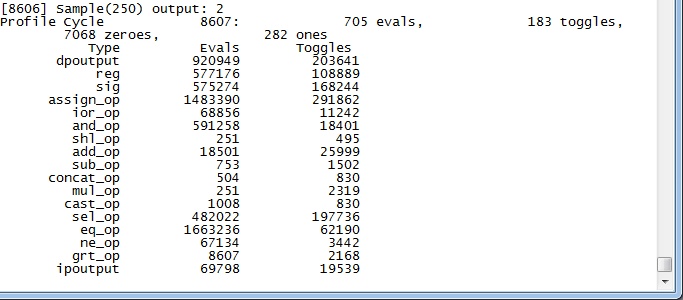
\includegraphics[width=1\textwidth]{Screenshots/Screenshot_Profiling.png}
			\caption{Screenshot of the toggle-profiling}
			\label{Toggles}
		\end{figure}
	

\section{Discussion}
	As shown in the performance analysis, the current setup with a processor and a co-processor takes 8606 clock cycles to calculate 250 data points (See figure \ref{Toggles}). Interestingly enough, this is actually slower than using the setup with a single processor - this setup were able to calculate the same amount of data points in only 7095 clock cycles. Even though this doesn't say anything about performance directly (Clock cycles times can vary, as specified in \nameref{Prob1}), the fact that the co-processor and the processor still has the same critical path, calculation wise (they perform the same calculations after all), it is clear that the setup with the co-processor is actually quite a bit slower. Furthermore, as described in \nameref{Performance Analysis}, the communication on the bus is actually one of the slowest parts of the setup, taking 8 clock cycles every time the processor has to load over the bus or send data over the bus to the co-processor. When comparing this to the fact that the actual calculations are quite simple (they can be done in a single clock cycle), it becomes clear that the bus is actually the current bottleneck of the system.\\
	\\
	Furthermore, this report identified several improvements that could be implemented in the final version of the ECG scanner - however, they are not implemented here as they required too much time compared to the deadline of this report. These improvements can be found in the section below.
	%Write all things bus-related here

	\subsection{Improvements}
		One improvement could be to implement simultaneous loading and data passing - that is, that the processor would be able to pass the data to the co-processor and then immediately start loading the next data point, as this is the process that takes the longest (8 clock cycles in Gezel). This could be done by implementing a dataStart and a dataEnd signal, used to synchronize the processor and the co-processor so the co-processor doesn't start to pass data back to the processor while the processor is loading the next data point.\\
		\\
		Alternatively, another improvement could be to implement the co-processor such that it would communicate directly with the processor, rather than using a bus. This would free up the bus to be used for the processors loading while the data is passed directly between the processor and co-processor.\\
		\\
		Furthermore, the co-processor could be improved more in terms of speed by storing the previous 30 values used for computation in the co-processor itself, rather than loading the old data. This would increase the size of the co-processor, but as this report focuses on improvements in terms of speed, this increase in size would be acceptable, considering that it remove a Load command which in itself takes 8 clock cycles (which is quite a great deal, considering that calculating an entire data point takes 35 clock cycles with the current operations).\\
		\\
		Improvements in terms of size could also be made by making a few assumptions, much like the one done with the data signal that goes between the processor and co-processor, but as this report focuses mainly on improving the speed, these have not been implemented yet. These improvements would simply be to reduce the bitwidth of various registers.\\
		

\section{Conclusion}
A co-processor were developed for the ECG scanner, optimized in the term of speed > power > size, as this were identified to be the order of importance for the performance. This report also identified that with the current bus-implementation, implementing a separate co-processor isn't a good idea as it actually decreases performance.

\newpage
\begin{thebibliography}{9}

\bibitem{A3}
  Michael Reibel Boesen, Jan Madsen, Linas Kaminskas, Karsten Juul Frederiksen, Thomas K. Malowanczyk\\
  \emph{Assignment 3: Implementation of an ECG co-processor}\\
  2013.\\

\bibitem{Gezel}
  \emph{Lecture7: Finite state machine with Datapath}\\
  Fall, 2007.\\

\bibitem{GezelBasicSyntax}
  \emph{GEZEL Basic Syntax}\\
  
\bibitem{CoreI5}
  \emph{\url{http://ark.intel.com/products/76088/Intel-Core-i7-4960HQ-Processor-6M-Cache-up-to-3\_80-GHz}}\\
  Used to determine size of the onboard memory of a Core I7
  
\end{thebibliography}
	
\newpage	
	\begin{Large}
		\textbf{Appendix}
	\end{Large}
	\appendix

\section{Who wrote what}
\underline{Jacob Gjerstrup, s113440 wrote:}\\
\textbf{Report: Abstract, Introduction, Analysis, Implementation (Good performance and Functionality of the co-processor), performance analysis, discussion, conclusion.}\\
\\
\underline{Jakob Welner, s124305 wrote:} \\
\textbf{Report: Design, Implementation (Communication and Implementation/Integration of the co-processor)}\\
\textbf{Code: Assembler code, coprocessor, Platform}

\section{Data files}
	\label{Commands}
	\lstinputlisting[language=Python]{Code/showCmds.txt}


\section{Sourcecode}

\subsection{Source code}
	\subsection{Assembly code}
		Python code:
		\lstinputlisting[language=Python]{Code/assembler.py}
		
		Assembler code for the program:
		\lstinputlisting{Code/assembler_program.txt}	
	
	\subsubsection{Co-processor}
		\lstinputlisting[language=C]{Code/coprocessor.fdl}
		
	\subsection{Platform code with co-processor integrated}
		\lstinputlisting[language=C]{Code/Platform.fdl}
	
	\subsection{Hexcodes for the program}
		\lstinputlisting{Code/program.txt}
\end{document}